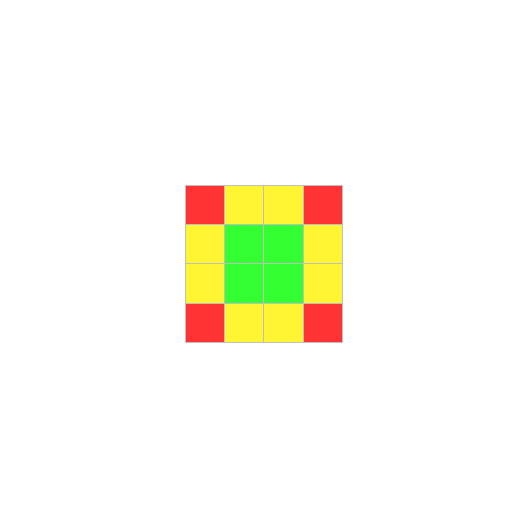
\begin{tikzpicture}[scale = 0.5]
    \def \Dx {12}
    \def \stp {1}
    \def \stpp {3}
  
    % style of grid
    \tikzset{gridstyle1/.style={color=lightgray,thin}}
    \tikzset{gridstyle2/.style={color=black,line width=1pt}}
    \tikzset{vertstyle1/.style={fill=red!80}}
    \tikzset{edgestyle1/.style={fill=yellow!80}}
    \tikzset{facestyle1/.style={fill=green!80}}

    \fill[color=white] (0, 0) rectangle (12*\stp, 12*\stp);
    \fill[style=edgestyle1] (4*\stp, 4*\stp) rectangle (8*\stp, 8*\stp);
    \fill[style=facestyle1] (5*\stp, 5*\stp) rectangle (7*\stp, 7*\stp);
    \fill[style=vertstyle1] (4*\stp, 7*\stp) rectangle (5*\stp, 8*\stp);
    \fill[style=vertstyle1] (4*\stp, 4*\stp) rectangle (5*\stp, 5*\stp);
    \fill[style=vertstyle1] (7*\stp, 4*\stp) rectangle (8*\stp, 5*\stp);
    \fill[style=vertstyle1] (7*\stp, 7*\stp) rectangle (8*\stp, 8*\stp);
    % \fill[style=vertstyle1] (0, 4*\stp) rectangle (1*\stp, 5*\stp);
    % \fill[style=vertstyle1] (4*\stp, 4*\stp) rectangle (5*\stp, 5*\stp);
    \draw[style=gridstyle1] (4*\stp, 4*\stp) grid (8*\stp, 8*\stp);
  
    % \draw[style=edgestyle1] (0, 0) rectangle (\stp, 12*\stp);
    % \draw[style=edgestyle1] (4*\stp, 0) rectangle (5*\stp, 12*\stp);
    % \draw[style=edgestyle1] (7*\stp, 0) rectangle (8*\stp, 12*\stp);
    % \draw[style=edgestyle1] (11*\stp, 0) rectangle (12*\stp, 12*\stp);
  
    % \draw[style=edgestyle1] (0, 0) rectangle (12*\stp, \stp);
    % \draw[style=edgestyle1] (0, 4*\stp) rectangle (12*\stp, 5*\stp);
    % \draw[style=edgestyle1] (0, 7*\stp) rectangle (12*\stp, 8*\stp);
    % \draw[style=edgestyle1] (0, 11*\stp) rectangle (12*\stp, 12*\stp);
  
  
  
    % \draw[style=vertstyle1] (0, 0) rectangle (\stp, \stp);0
    % \draw[style=vertstyle1] (4*\stp, 0) rectangle (5*\stp, \stp);
    % \draw[style=vertsty0le1] (7*\stp, 0) rectangle (8*\stp, \stp);
    % \draw[style=vertstyle1] (11*\stp, 0) rectangle (12*\stp, \stp);
  
    % \draw[style=vertstyle1] (0, 4*\stp) rectangle (\stp, 5*\stp);
    % \draw[style=vertstyle1] (4*\stp, 4*\stp) rectangle (5*\stp, 5*\stp);
    % \draw[style=vertstyle1] (7*\stp, 4*\stp) rectangle (8*\stp, 5*\stp);
    % \draw[style=vertstyle1] (11*\stp, 4*\stp) rectangle (12*\stp, 5*\stp);
  
    % \draw[style=vertstyle1] (0, 7*\stp) rectangle (\stp, 8*\stp);
    % \draw[style=vertstyle1] (4*\stp, 7*\stp) rectangle (5*\stp, 8*\stp);
    % \draw[style=vertstyle1] (7*\stp, 7*\stp) rectangle (8*\stp, 8*\stp);
    % \draw[style=vertstyle1] (11*\stp, 7*\stp) rectangle (12*\stp, 8*\stp);
  
    % \draw[style=vertstyle1] (0, 11*\stp) rectangle (\stp, 12*\stp);
    % \draw[style=vertstyle1] (4*\stp, 11*\stp) rectangle (5*\stp, 12*\stp);
    % \draw[style=vertstyle1] (7*\stp, 11*\stp) rectangle (8*\stp, 12*\stp);
    % \draw[style=vertstyle1] (11*\stp, 11*\stp) rectangle (12*\stp, 12*\stp);
  
    % % \draw[fill=red!30,draw=white] (\stp*2,\stp*2) rectangle (\stp*3,\stp*3);
    % \draw[style=gridstyle1,step=\stp] (0,0) grid (\Dx,\Dx);
    % \draw[style=gridstyle2,step=\stpp] (0,0) grid (\Dx,\Dx);
  
    % \draw plot coordinates{(\stp*2+\stp/2,\stp*2+\stp/2)} node[sloped] {$\Omega_{i}$};
    % \draw[line width=2pt,color=blue] (\Dx/2, 0) -- (0,0) -- (0,\Dx) -- (\Dx/2,\Dx);
    % \draw[line width=2pt,color=red] (\Dx/2, 0) -- (\Dx,0) -- (\Dx,\Dx) -- (\Dx/2,\Dx);
    % \draw[->, ultra thick] (-2,\Dx/2+1) node[sloped, left]{$\Gamma_{D}$} -- (0,\Dx/2);
    % \draw[->, ultra thick] (\Dx+2,\Dx/2+1) node[sloped, right]{$\Gamma_{N}$} -- (\Dx,\Dx/2);
    % \draw[fill=yellow!50] (0.5,0.5) circle (0.2);
    % \draw plot [mark=*, mark size=2] coordinates{(0.5,0.5)};
    % \draw[fill=yellow!50] (\Dx-0.5,\Dx-0.5) circle (0.2);
    % \draw plot [mark=*, mark size=2] coordinates{(\Dx-0.5,\Dx-0.5)};
    % \draw[->, ultra thick] (-1,1) node[sloped, left]{$\Gamma_{I}$} -- (0.5,0.5);
    % \draw[->, ultra thick] (\Dx+0.5,\Dx+0.5) node[sloped, right]{$\Gamma_{P}$} -- (\Dx-0.5,\Dx-0.5);
  \end{tikzpicture}
  